\chapter{均衡理论}
\setlength{\parskip}{0.5\baselineskip}

对于经济学,图像是重要的;对于图像,坐标轴的变量是重要的,同时各种变量是经济学的研究目标,这就要求我们在看图的时候不能忽视“坐标轴代表的变量是什么”。从第一章开始我们就会接触图像,学习一种曲线时,我们要本能地去关注它代表的是哪两个对应变量构成的轨迹,这样的学习方法可以帮助我们深刻地理解经济学曲线。

\section{需求}

\subsection{需求量}

\begin{dingyi}[breakable]{需求量}
    啊在其他因素不变时,消费者在一定价格水平下愿意且能够支付的该商品数量。
\end{dingyi}

需求量的定义中体现了单个价格水平与单个商品数量的对应关系。这里“价格水平”是一个巧妙的表达,我们不仅可以研究某款特定电脑的在确定价格时消费者的需求量,也可以研究整个电脑行业的价格水平(比如取所有电脑价格的平均数作为价格水平)对应的消费者需求量,体现了使用价格水平来表达的重要性。

\subsection{需求}

\begin{dingyi}[breakable]{需求}
    啊在其他因素不变时,消费者在一定时期内对于各种可能价格水平愿意且能够支付的该商品数量。
\end{dingyi}

在需求量的基础上,我们得到需求的定义,开始考虑多种价格水平。根据定义,当得知消费者在各种价格水平下的需求量,便可以知道消费者对商品的需求。在这句话中就出现了“需求量”三个字,说明需求是由需求量构成的。既然我们掌握了价格水平与需求量的对应关系,这不正是在章首提到的“曲线是两个对应变量构成的轨迹”,就能画出需求曲线了。需求曲线上的每一个点都是消费者的需求量。

对比需求量和需求的定义,不难发现如“包子变贵后需求变小了”是不准确的表达,因为与特定价格对应的是定义是需求量。虽然在表达中严格区分需求和需求量是有助于读者理解的做法,但也会增加作者的工作量,所以往后多数语义明确的场合,本书将混淆需求和需求量,统称为“需求”。

\subsection{需求函数}

\begin{dingyi}[breakable]{需求函数}
    啊在其他因素不变时,简化版的需求函数为 $Q^d=f\left(P\right)$;更为复杂的马歇尔需求函数为 $Q_d=f\left(P_X,P_Y,I\right)$,其中 $P_X$ 为本商品价格,$P_Y$ 为其他商品价格,$I$ 为收入。
\end{dingyi}

马歇尔一派认为除了本商品价格会决定消费者的需求量,其他商品的价格和消费者的收入也会左右需求量,这是符合直觉的。

\subsection{影响需求量的因素}

影响需求量的因素有以下几种
\begin{enumerate}
    \item 自身商品价格(需求函数的自变量)
    \item 相关商品价格(需求函数的自变量)
    \item 消费者收入水平(需求函数的自变量)
    \item 消费者的预期
    \item 消费者的偏好
    \item 政策风向
    \item ……
\end{enumerate}

需求函数的自变量是需求量的决定性变量,毫无疑问会影响需求量。图 1-1 中,我们忽略其他商品价格和收入的影响,把本商品价格和对应的需求量画出来,得到结论:价格下降会伴随需求量下降,这是“点移动”。如果价格以外的因素导致需求量变化,即任意价格水平不变时需求量发生变化,则会发生“线移动”。有这样的区别,是因为价格是需求函数的内生变量,其他因素是需求函数的外生变量,即使马歇尔需求函数认为其他商品价格和收入也是需求的决定性因素,但在这里被我们抛弃了,也成为了影响需求曲线移动的外生变量。

综上所述,价格因素变动会引起需求量变动,非价格因素不仅会引起需求量变动,还会引起整个需求曲线移动。这样的分析方法还适用于其他许多场合,尤其是判断移动类型。

\begin{figure}[H]
    \centering
    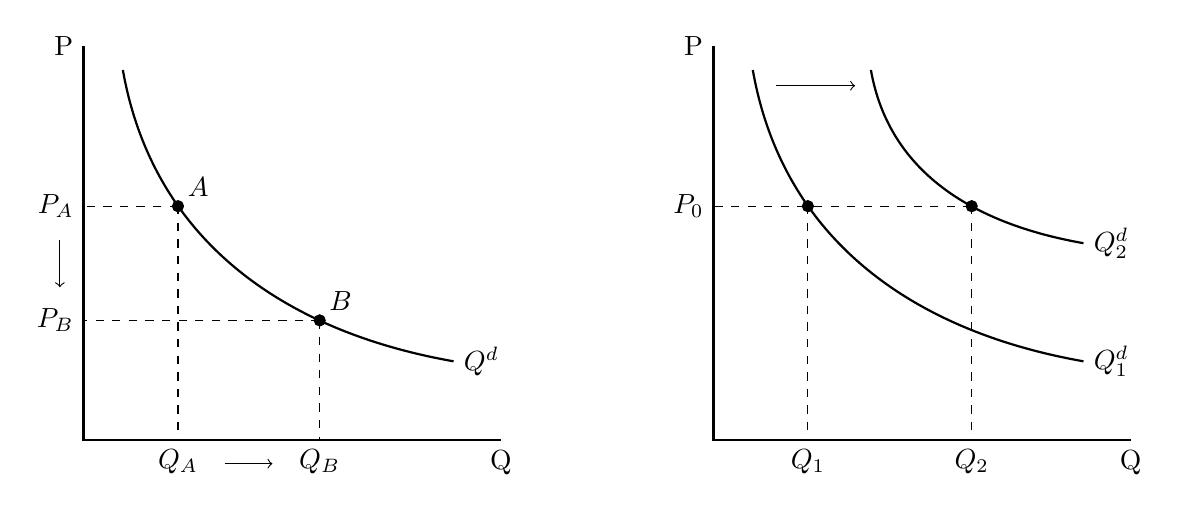
\begin{tikzpicture}
        \draw[thick] (0,5) node[left]{$\rm P$} -- (0,0) -- (5.3,0) node[below]{$\rm Q$};
        \draw[thick] (0.5,4.7) to [out=280,in=170](4.7,1) node[right]{$Q^d$};
        \filldraw[black] (1.2,2.97) circle (2pt) node[above right]{$A$};
        \filldraw[black] (3,1.52) circle (2pt) node[above right]{$B$};
        \draw[dashed] (1.2,2.97) -- (1.2,0) node[below]{$Q_A$};
        \draw[dashed] (1.2,2.97) -- (0,2.97) node[left]{$P_A$};
        \draw[dashed] (3,1.52) -- (3,0) node[below]{$Q_B$};
        \draw[dashed] (3,1.52) -- (0,1.52) node[left]{$P_B$};
        \draw[->] (1.8,-0.3) -- (2.4,-0.3);
        \draw[->] (-0.3,2.54) -- (-0.3,1.94);
    \begin{scope}[xshift=8cm]
        \draw[thick] (0,5) node[left]{$\rm P$} -- (0,0) -- (5.3,0) node[below]{$\rm Q$};
        \draw[thick] (0.5,4.7) to [out=280,in=170](4.7,1) node[right]{$Q^d_1$};
        \draw[thick] (2,4.7) to [out=280,in=170](4.7,2.5) node[right]{$Q^d_2$};
        \draw[->] (0.8,4.5) -- (1.8,4.5);
        \filldraw[black] (1.2,2.97) circle (2pt);
        \filldraw[black] (3.28,2.97) circle (2pt);
        \draw[dashed] (1.2,2.97) -- (1.2,0) node[below]{$Q_1$};
        \draw[dashed] (3.28,2.97) -- (3.28,0) node[below]{$Q_2$};
        \draw[dashed] (3.28,2.97) -- (0,2.97) node[left]{$P_0$};
    \end{scope}
    \end{tikzpicture}
\caption{需求量变动}
\end{figure}

\begin{mantan}[breakable]{我们如何作图?}
    啊经济学中的作图与数学中的有较大不同。一个被公认的马歇尔坐标系被允许不画箭头和原点,自变量在纵轴,因变量在横轴。如果你画出箭头和原点是无可厚非的,没人在乎这么多,但坐标轴绝不能画反。画图是经济学学生的基本功,应勤加练习,熟练掌握课本中的图像绘制。
\end{mantan}

\section{供给}

\subsection{供给量}

\begin{dingyi}[breakable]{供给量}
    啊在其他因素不变时,生产者在一定价格水平下愿意且能够生产的该商品数量。
\end{dingyi}

\subsection{供给}

\begin{dingyi}[breakable]{供给}
    啊在其他因素不变时,生产者在一定时期内对于各种可能价格水平愿意且能够生产的该商品数量。
\end{dingyi}

\subsection{供给函数}

\begin{dingyi}[breakable]{供给函数}
    啊在其他因素不变时,简化版的供给函数为 $Q^s=f\left(P\right)$。
\end{dingyi}

一般来说,供给函数是递增的,需求函数是递减的,所以供给函数比需求函数更应该关心价格轴上的截距,避免价格出现负数。

\begin{mantan}[breakable]{我们为什么研究供给?}
    啊虽然供给函数的形式比需求函数的简单,但微观经济学的市场理论中会对供给函数展开大篇幅的讨论。消费者的需求量来自于偏好,而且消费目标是效用最大化,效用是一种感觉,这些要素几乎是无迹可寻的(用金钱度量效用可能会遭到道德批判);生产者的供给量来自于收益与成本的考量,有明确的利润最大化目标,这在方法论上说明了研究供给的可行性。另一方面厂商是利益共同体,消费者是分散个体,一个市场内的消费者数量往往比厂商数量多得多。人们可以后悔今天早上不该多买个包子,而厂商经不起决策失误,这是说明了研究供给的重要性。
    
    当然,需求不是不重要,需求不是不用研究。在消费者领域,我们更关心需求背后的逻辑,如偏好和选择,用数学工具对这些主题进行研究可以得到需求函数。
\end{mantan}

\subsection{影响供给量的因素}

影响供给量的因素有以下几种

\begin{enumerate}
    \item 自身商品价格(供给函数的自变量
    \item 生产成本水平
    \item 生产技术水平
    \item 相关商品价格
    \item 生产者的预期
    \item 政策风向
    \item ……
\end{enumerate}

\section{市场均衡}

\begin{dingyi}[breakable]{均衡}
    啊经济事物中有关变量在一定条件的相互作用下所达到的一种相对静止的状态。
\end{dingyi}

均衡的定义中“相对静止”可以理解为“没有一个经济主体愿意改变”,这可以引申出丰富的含义。以下是帮助理解“均衡是什么”的例子:

\begin{enumerate}
    \item 小明是素食主义者,永远不吃肉,这是均衡
    \item 两个厂商达成共识,把商品价格定在 10 元,这是均衡
    \item 宏观经济中等于贸易余额资本净流出($NX=CF$),这是均衡
    \item 超长期中资本存量有稳态,$\Delta k=0$,在图像上 $k^*$ 固定不动,这是均衡
    \item 下一期的价格 $P_{t+1}$ 按照 $P_{t+1}=f\left(P_t\right)$ 迭代,最终收敛到一个固定值,这是均衡
\end{enumerate}

需求曲线上的点都是消费者的均衡,供给曲线上的点都是生产者的均衡,两者相交的点是市场的均衡。竞争性均衡有要求:1. 不存在市场势力;2. 消费者效用最大化;3. 生产者利润最大化;4. 市场出清。

\section{弹性}

\subsection{弹性的基本定义}

\begin{dingyi}[breakable]{弹性}
    啊在其他因素不变时,一个变量变动 1\% 所引起另一个变量变动百分比。
    \vspace{0.5em}
    
    记号:$E$;公式:$E_{YX}=\dfrac{\%\Delta Y}{\%\Delta X}=\dfrac{\Delta Y\,/\,Y}{\Delta X\,/\,X}$($\%\Delta$ 为变动百分比的符号)
    \vspace{0.5em}
    
    点弹性:$E_{YX}=\dfrac{\mathrm dY}{\mathrm dX}\cdot\dfrac XY$ \quad\quad 弧弹性:$E_{YX}=\dfrac{\Delta Q}{\Delta P}\cdot\dfrac{\left(P_1+P_2\right)\,/\,2}{\left(Q_1+Q_2\right)\,/\,2}$
\end{dingyi}

关于弹性的定义,有许多注意点:

\begin{enumerate}
    \item 定义表达式比具体公式更重要,它可以帮助我们快速分辨弹性大小
    \item 自变量放在分母,因变量放在分子。弹性记号的下角标中,前者是分子,后者是分母,如 $E_{YX}$ 表示 $X$ 变动引起 $Y$ 变动的弹性
    \item 计算点弹性只需要需求函数形式与一组价格和需求的数据,计算弧弹性不需要需求函数形式,需要两组数据,这是它们的区别。如果给了两组数据 $\left(P,Q\right)_{\text{前}}$ 和 $\left(P,Q\right)_{\text{后}}$ 并要求计算点弹性,则使用变动前的数据 $\left(P,Q\right)_{\text{前}}$
    \item 弧弹性比点弹性的精确度更高,但当两种弹性都能计算出来时,优先计算点弹性
    \item 公式的表达式都是形式!不同的书可能有不同的形式,所以不要奇怪为什么有时候看到不同的公式
    \item 公式中是否带有负号也是不同教材采取不同做法导致的迷惑,所以不要纠结于要不要带负号,根据自己使用的教材决定是否加符号
\end{enumerate}

\begin{mantan}[breakable]{我们为什么不用导数?}
    啊从引入弹性开始,我们要开始研究一个变量变动对另一个变量的影响了。固定住其他因素是很自然的做法,如果不这么做,会导致 $Y$ 的变动中分不清多少由 $X$ 变动引起。导数 $\mathrm dY/\mathrm dX$ 也可以胜任这个任务,但我们拒绝使用导数,而是弹性 $\%\Delta Y/\%\Delta X$,是因为百分比变动可以消除量纲的影响。同样一个经济变量,使用不同的单位会得到不同绝对数值变化,从而得到不同的导数值,这种情况是在使用变化百分比中不会出现的。
\end{mantan}

\subsection{弹性的种类}

因为点弹性是重要的,所以我们选择点弹性作为以下弹性种类的公式。

\begin{dingyi}[breakable]{各类弹性}
    啊需求的价格弹性:$E_{P}=\dfrac{\mathrm dQ}{\mathrm dP}\cdot\dfrac{P}{Q}$ \quad\quad 需求的收入弹性:$E_{I}=\dfrac{\mathrm dQ}{\mathrm dI}\cdot\dfrac{I}{Q}$
    \vspace{0.5em}

    需求的交叉弹性:$E_{XY}=\dfrac{\mathrm dQ_X}{\mathrm dP_Y}\cdot\dfrac{P_Y}{Q_X}$ \quad\quad 供给的价格弹性:$E_{P}=\dfrac{\mathrm dQ}{\mathrm dP}\cdot\dfrac{P}{Q}$
\end{dingyi}

在经济学中,我们要像在数学中使用导数一样使用弹性,以上只列举了部分弹性类型,往后会见到更多种类。

这里我们还要注意:经济学的坐标轴与数学的相反,我们看到的曲线表达式实际是 $P=f^{-1}\left(Q\right)$,所以对斜率的判断也要相反,$\mathrm dQ/\mathrm dP$ 很大理应是陡峭,但在图像上直接看到的是平坦。有了这个经验,我们在对比两条曲线的弹性时,可以用个小结论:曲线越平坦,弹性越大;曲线越陡峭,弹性越小。极端时,曲线垂直于横轴,弹性为零;曲线平行于横轴,弹性为无穷大。

\begin{tuxiang}[breakable]{线性需求函数的弹性}
    啊虽然线性需求函数的导数是不变的,但弹性是会变的,图中的箭头标示:从右下角到左上角,弹性逐渐变大。其中曲线在第一象限的中点 $\left(P_0/2,Q_0/2\right)$ 的弹性 $E_P=1$。
\end{tuxiang}
\begin{figure}[H]
    \centering
    \includegraphics[width=0.4\textwidth]{1 price elasticity of demand on linear curve.jpg}
\end{figure}

\begin{shuxue}[breakable]{单位弹性时销售收益最大化}
    啊对于某商品而言,它的单价是固定的,所以销售收益为$TR=P\,Q$。销售收益对价格求导得最优化一阶条件
    $$\frac{\mathrm{d}TR}{\mathrm{d}P}=Q+P\,\frac{\mathrm{d}Q}{\mathrm{d}P}=Q\left( 1+\frac{\mathrm{d}Q}{\mathrm{d}P}\frac{P}{Q} \right) =Q\left( 1-E_P \right)=0$$
    $E_P=1$ 满足一阶条件,证毕。
\end{shuxue}

\subsection{商品分类}

\noindent\textbf{按需求的价格弹性分类}
\begin{enumerate}
    \item 普通品:$\dfrac{\mathrm dQ}{\mathrm dP}>0$,$E_P>0$
    \item 吉芬品:$\dfrac{\mathrm dQ}{\mathrm dP}<0$,$E_P<0$
\end{enumerate}
\vspace{1em}

\noindent\textbf{按需求的收入弹性分类}
\begin{enumerate}
    \item 正常品:$\dfrac{\mathrm dQ}{\mathrm dI}>0$,$E_I>0$
    \begin{enumerate}
        \item 奢侈品:$E_I>1$(注意不对导数作要求)
        \item 必需品:$E_I<1$(注意不对导数作要求)
    \end{enumerate}
    \item 奢侈品:$\dfrac{\mathrm dQ}{\mathrm dI}<0$,$E_I<0$
\end{enumerate}
\vspace{1em}

\noindent\textbf{按需求的交叉价格弹性分类}
\begin{enumerate}
    \item 替代品:$E_{XY}>0$
    \item 互补品:$E_{XY}<0$
\end{enumerate}

\subsection{长短期中的弹性}

\noindent\textbf{供给价格弹性}(短期 < 长期)
\begin{enumerate}
    \item 短期:受到生产能力的约束,产量可变化范围不大
    \item 各种要素可以自由调节投入量,产量可变化范围相比短期大很多,同时企业可以调整规模、重组生产要素,以降低成本,生产出更多产品
\end{enumerate}
\vspace{1em}

\noindent\textbf{非耐用品的需求价格弹性}(短期 < 长期)
\begin{enumerate}
    \item 短期:消费者偏好比较稳定,虽然价格升高,人们还是按照习惯购买同样数量的商品
    \item 长期:消费者偏好改变,或者找到更合适的替代品,就会改变对原商品的需求量
\end{enumerate}
\vspace{1em}

\noindent\textbf{耐用品的需求价格弹性}(短期 > 长期)
\begin{enumerate}
    \item 短期:因为其使用周期较长,若价格上升,消费者需求量骤减,使用之前购买的耐用品;若价格下降,消费者需求量骤增,趁机囤货
    \item 长期:消费者对耐用品的需求量比较稳定,如小轿车,当一个家庭里已经拥有了一辆小轿车后,少有因为小轿车价格下降而再购买一辆
\end{enumerate}
\vspace{1em}

\zhu 收入上升相当于商品价格下降,因此需求收入弹性的分析类似于需求价格弹性的。